% mnras_template.tex
%
% LaTeX template for creating an MNRAS paper
%
% v3.0 released 14 May 2015
% (version numbers match those of mnras.cls)
%
% Copyright (C) Royal Astronomical Society 2015
% Authors:
% Keith T. Smith (Royal Astronomical Society)

% Change log
%
% v3.0 May 2015
%    Renamed to match the new package name
%    Version number matches mnras.cls
%    A few minor tweaks to wording
% v1.0 September 2013
%    Beta testing only - never publicly released
%    First version: a simple (ish) template for creating an MNRAS paper

%%%%%%%%%%%%%%%%%%%%%%%%%%%%%%%%%%%%%%%%%%%%%%%%%%
% Basic setup. Most papers should leave these options alone.
\documentclass[fleqn,usenatbib]{mnras}  % a4paper,

% MNRAS is set in Times font. If you don't have this installed (most LaTeX
% installations will be fine) or prefer the old Computer Modern fonts, comment
% out the following line
%\usepackage{newtxtext,newtxmath}
\usepackage{txfonts}
% Depending on your LaTeX fonts installation, you might get better results with one of these:
%\usepackage{mathptmx}
%\usepackage{txfonts}


% Use vector fonts, so it zooms properly in on-screen viewing software
% Don't change these lines unless you know what you are doing
\usepackage[T1]{fontenc}
\usepackage{ae,aecompl}
\usepackage{slashbox}

%%%%% AUTHORS - PLACE YOUR OWN PACKAGES HERE %%%%%

% Only include extra packages if you really need them. Common packages are:
\usepackage{graphicx}	% Including figure files
\usepackage{amsmath}	% Advanced maths commands
\usepackage{amssymb}	% Extra maths symbols

%%%%%%%%%%%%%%%%%%%%%%%%%%%%%%%%%%%%%%%%%%%%%%%%%%

%%%%% AUTHORS - PLACE YOUR OWN COMMANDS HERE %%%%%

% Please keep new commands to a minimum, and use \newcommand not \def to avoid
% overwriting existing commands. Example:
%\newcommand{\pcm}{\,cm$^{-2}$}	% per cm-squared

%%%%%%%%%%%%%%%%%%%%%%%%%%%%%%%%%%%%%%%%%%%%%%%%%%

%%%%%%%%%%%%%%%%%%% TITLE PAGE %%%%%%%%%%%%%%%%%%%

% Title of the paper, and the short title which is used in the headers.
% Keep the title short and informative.
\title[Quasar Variability]{Solving the puzzle of discrepant variability on monthly time scales implied by SDSS and CRTS datasets}

% The list of authors, and the short list which is used in the headers.
% If you need two or more lines of authors, add an extra line using \newauthor
\author[K. Suberlak et al.]{
Krzysztof Suberlak,$^{1}$\thanks{E-mail: suberlak@uw.edu}
\v{Z}eljko Ivezi\'c, $^{1}$
Chelsea L. MacLeod,$^{2}$
Matthew Graham,$^{3}$ 
\newauthor
$\, \,  $Branimir Sesar$^{4}$
\\
% List of institutions
$^{1}$Department of Astronomy, University of Washington, Seattle, WA, United States\\
$^{2}$Institute for Astronomy, University of Edinburgh, Royal Observatory, Edinburgh, United Kingdom\\
$^{3}$Center for Data-Driven Discovery, California Institute of Technology, Pasadena, CA, United States\\
$^{4}$National Optical Astronomy Observatory, Tucson, AZ, United States.
}

% These dates will be filled out by the publisher
\date{Accepted XXX. Received YYY; in original form ZZZ}

% Enter the current year, for the copyright statements etc.
\pubyear{2015}

% Don't change these lines
\begin{document}
\label{firstpage}
\pagerange{\pageref{firstpage}--\pageref{lastpage}}
\maketitle

% Abstract of the paper
\begin{abstract}

We present improved error analysis for the 3,800 CRTS (Catalina Real-Time Transient Survey) optical quasar light curves from the Sloan Digital Sky Survey Stripe 82 catalog. SDSS imaging survey has provided a time-resolved photometric  dataset which greatly improved our understanding of the quasar optical continuum variability: data for monthly and longer timescales  are consistent with a damped random walk. Recently, newer data  obtained by CRTS (Catalina Real-Time Transient Survey) provided  puzzling evidence for enhanced variability, compared to SDSS results, on monthly time scales. Quantitatively, SDSS results predict  about $0.06$ mag rms variability for timescales below 50 days, while CRTS data show about a factor of two larger root-mean-square  for spectroscopically confirmed SDSS quasars. Our analysis presented here has successfully resolved this discrepancy as due to slightly underestimated photometric error estimates provided by the CRTS image processing pipelines. The photometric error correction factors, derived from detailed analysis of non-variable SDSS standard stars that were re-observed by CRTS, are about $20-30\%$, and result in a quasar variability behavior implied by the CRTS data fully consistent with earlier SDSS results.


\end{abstract}


%%%%%%%%%%%%%%%%%%%%%%%%%%%%%%%%%%%%%%%%%%%%%%%%%%

%%%%%%%%%%%%%%%%% BODY OF PAPER %%%%%%%%%%%%%%%%%%

\section{Introduction}
\label{sec:intro}

Quasar variability is an important characteristic that has a potential to shed light on the structure of the innermost region of the accretion disk, and has been the subject of research for the past half century (Matthew, Sandage 1963, Vanden Berk + 2004, Grier+2012, Kozlowski+2016). The Sloan Digital Sky Survey (SDSS, Schmidt+2010, Sesar+2007) and Catalina Real-Time Transient Survey (CRTS, Djorgovski+2012, Drake+2009) allowed an unprecedented study of well-calibrated light curves. 

Assuming that the observed  variability of a lightcurve -   discretely sampled time series -  is caused by a continuous underlying physical phenomenon, to characterise it we can use a mathematical formalism of a stochastic process model (Kasliwal+2015). A one-parameter Auto-Regressive, AR(1), process  may correspond to the physical situation of an environment where a disturbance is diffused and returns to the median value. Various explanations exist for the nature of such disturbances,  including supernovae, microlensing, accretion disk instabilities, and thermal fluctuations  (Kelly+2009, Kelly+2011, Collier\&Peterson 2001, Ruan+2014).  Most likely, thanks to  Reverberation Mapping studies (Peterson 2004, Fausnaugh+2016,  Munoz+2016), we understand the accretion disk to be  the main source of the underlying variability. 

At the cadence of the CRTS survey (more than few days), the AR(1) process (Damped Random Walk model) describes well the quasar variability ( Butler & Bloom 2011, MacLeod+2010,2011,2012, Kelly+2009, Zu+2011,2013, Kozlowski+2010a, Ruan+2012).  [A deviation from the DRW model at very short timescales, reported by Kasliwal+2015, is based on Kepler lightcurves at cadences shorter than a day, which is below the observational limit of CRTS. For this reason, in this paper DRW is assumed to be a good descriptor of the quasar stochastic variability].
 
The DRW model has two parameters - an amplitude of variability, and a characteristic timescale, that corresponds to the timescale of damping of thermal oscillations or orbital timescale (Kelly+2009).   When the lightcurves are sparsely sampled,  it is more meaningful to describe their ensemble properties,  using the structure function (SF), which is  well defined for a collection of variable objects driven by the DRW (Kozlowski+2010, 2016, Vanden Berk+2004, Schmidt+2010, Hawkins+2002)

 Recent SDSS-based studies (MacLeod+2010, Kelly+2009) reflect the traditional timescale of $\tau > 100 $ days in quasar rest frame, supported by OGLE results of Zu+2014 with $ 17 \leq \tau \leq 2700 $ days. However, a CRTS-based study of Graham+2014 that used Slepian Wavelet Variance methodology found $\tau ~ 54$ days. The latter is consistent with the Kepler-based results of Kasliwal+2015 for cadences above a day, who found   $ 17 \leq \tau \leq 2700 $ days.  The aim of this paper is to revisit the analysis of the CRTS quasars using a  well-tested approach of the Structure Function, and detailed error analysis (MacLeod+2010, MacLeod+2012, Simonetti+1984, Vanden Berk+2004, Sumi+2005, Bauer+2009). 
 
In section \ref{sec:obs} we describe the properties of our dataset, all selection criteria, and the structure function analysis.  In section \ref{sec:err_analysis} we explain the results of our analysis of the small timescale subset of the structure function. This is followed by discussion of the impact of our result, and conclusions in sections \ref{sec:discussion} and \ref{sec:conclusions}.
 

\section{Data Analysis}
\label{sec:obs}

Catalina Real-time Transient Survey (CRTS) employed three telescopes ( "0.7 m Catalina Sky Survey Schmidt and 1.5 m Mount Lemmon Survey telescopes in Arizona, and the 0.5 m Siding Springs Survey Schmidt in Australia" Graham+2015), each with a  4kx4k CCD detector (Djorgovski+2011). All observations were taken in an unfiltered white light, and calibrated to the Johnson system V-band zero point (Drake+2013). In this research we use CRTS lightcurves of 7932 spectroscopically-confirmed QSOs and 52133 standard stars  from the equatorial region of the sky ($22h 24m < \mathrm{R.A.} < 04h 08m$ and $\mathrm{| Dec |} < 1.27 deg$)  known as the Stripe 82 (Sesar+2010). Our sampling criterion : more than 10 measurements per lightcurve, leaves 7707 quasars and 49385 stars.  To improve signal to noise we perform day-averaging, and thus we  also require more than 10 individual days of observations per lightcurve, leaving in the final sample 7601 quasars and 48250 stars (see Fig.\ref{fig:CRTS_QSO_stats} for statistical description of the quasar sample). 

We complement the CRTS data for each object  with the SDSS photometry by creating a positionally cross-matched catalog using astropy  \verb|match_to_catalog_sky| routine. For catalog matching we used the SDSS Stripe 82 standard stars catalog  ver. 2.6  (Ivezic+2007), and for  the SDSS DR7  Stripe 82 quasars catalog (Abazajian+2009).   Since the SDSS star catalog contains accurate data for 1006849 stars , all CRTS stars were found to have a matching SDSS counterpart within 0.01 arcsec.  Of 7601  CRTS quasars,  7586 had an SDSS counterpart within 0.36 arcsec.  The remaining 15 CRTS quasars had an SDSS counterpart within between  2 and 9 arcmin  [ - they were ignored ?  ]   

\begin{figure}
\label{fig:CRTS_QSO_stats}
 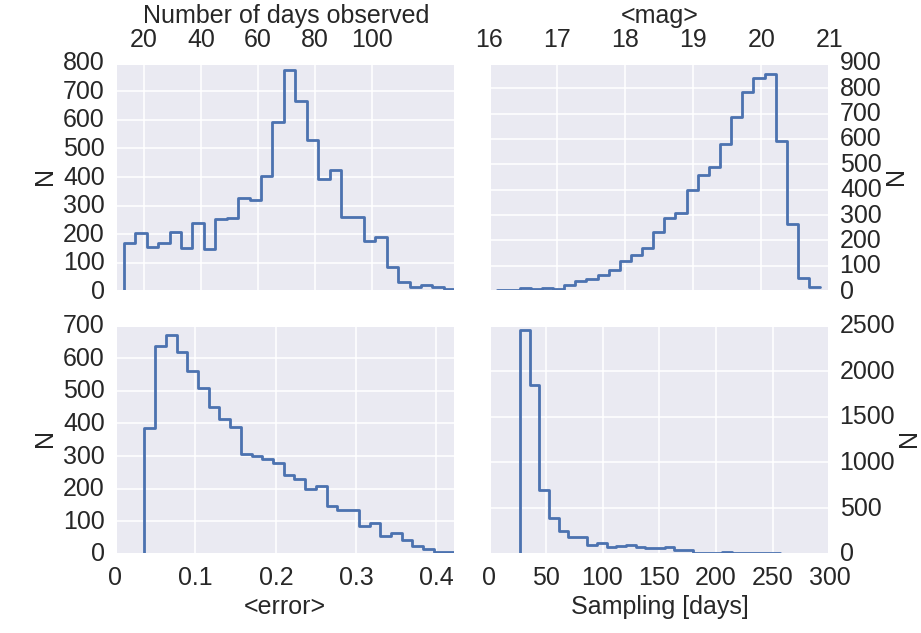
\includegraphics[width=\columnwidth]{Fig_1_Stats_CRTS_QSO_used.png}
 \caption{Statistical information about the CRTS QSO final sample of 7601 day-averaged light curves. The upper-left panel shows the number of days that a given quasar was observed, i.e. $max(MJD)-min(MJD)$ per light curve. The upper-right panel shows the average light curve magnitude. The bottom-left panel shows the light curve averaged error. If $i$, $i+1$ are two consecutive day-averaged observations in the light curve, then $MJD_{i} - MJD_{i+1}$ is the sampling interval. The bottom-right panel shows light curve - averaged sampling intervals. The light curve and sample-averaged mean and median error is 0.22. The mean  brightness is 19.50, and the mean number of individual observations per light curve  is 209. Within that sample , $96 \% $ observations of quasars span the time of 7-9 years.  $91.2\%$ of  quasars were observed between 1 to 4 times per night.}
\end{figure}


To improve the signal-to-noise ratio we performed day-averaging of light curves. The day-magnitude is the mean of individual measurements, and the day-error $e_{w}$ is the weighted sum of individual errors $e_{i}$: 

\begin{equation}
 e_{w} = \frac{1}{\sqrt[]{\sum_{i} w_{i}}}
\end{equation}

where $ w_{i} = 1 / e_{i}^{2}$ is the weight assigned to each point. To avoid unphysically small error values, we added  $0.01$ $mag$ to $e_{w}$ in quadrature if $e_{w}<0.02$ $mag$. [A typical sampling interval of day-averaged CRTS Quasar lightcurves is $\approx 20$ days.] 

\section{Structure Function}

The structure function is a well-studied approach to characterising quasar light curves. It describes the relationship between the time lag and the amplitude of brightness variability (Cristiani+1996, Schmidt+2010, Vanden Berk +2004, de Vries + 2005, Rengstorf + 2006). 

 Similarly to Schmidt+2010, we  calculate the structure function for all objects  using  the magnitude difference $\Delta m _{i,j}$ between light curve points $i$ and $j$, separated by a time lag $\Delta t_{i,j}$. To avoid the additional uncertainty of redshift estimates based on the SDSS spectra, we also use time lags in the observed frame. We add the error information in quadrature: $e_{ij} = \sqrt{e_{i}^{2}+e_{j}^{2}}$. Such 'master file' containing  

To analyze the magnitude difference  we bin the $\Delta m _{i,j}$ points from all objects  it in logarithmic $\Delta t_{i,j}$  space. The number of chosen bins is a choice of convenience between very coarse grid (a small number of bins) or a very fine grid, risking a small number of points per bin. Having performed tests  with $50$, $100$, $200$, $400$ bins we find that $N=200$ is the right choice between computational efficiency and information content. 

We calculate the $SF$ using an exact prescription involving marginalizing the log-likelihood of the probability in $p(SF)$ and $p(\mu)$ space per bin, after [Ivezic+2013], chapter 5: 
 
\begin{equation}
\centering
\frac{d p(SF}{d SF } \bigg| _{SF = mode} = 0
\end{equation}

For each bin we calculate four statistical descriptors, shown on Fig.~\ref{fig:panel_plots} -  standard deviation from the mean ($\sigma$, Gaussian robust deviation from the mean $\sigma_{G}=0.7414 (q_{75}-q_{25})$, the Structure Function ($SF$) and the mean ($\mu$).  

To show the departure of the CRTS quasars from the DRW model we fit to the $SF$ a  fiducial DRW  model:
\begin{equation}
SF(\Delta t) = SF_{\infty} \cdot \left( 1-e^{-\Delta t / \tau} \right) ^ {1/2}
\end{equation}

with model error $\sqrt{SF(\Delta t) ^ {2} + err_{SF} ^ {2}}$. 



\begin{figure}
\label{fig:panel_plots}
 \includegraphics[width=\columnwidth]{{Fig_2_18.5-19_panels_fc-1.0_NEW}.png}
 \caption{The four panels show statistics calculated for the subsample of 333 CRTS quasars (black points), 1400 "blue" stars (blue points), and 2087 "red" stars (red points), all  chosen according to the SDSS r magnitude $18.5 < \mathrm{m} < 19$.  For "red"  stars we require that SDSS colors are $1 < \mathrm{g-i} < 3$ and  for "blue" stars $-1 < \mathrm{g-i} < 1$. Lightcurve-derived  pairwise brightness differences for all objects of a given type are binned according to  linearly spaced $200$ bins in $\Delta_{t}$. The binning was not found to affect the main features of the plot.  The sine-like modulation reflects differences in number of points in each bin (from tens to hundreds of thousands per bin). For each bin, we calculated for each type of object the standard deviation $\sigma_{stdev}$, the robust Gaussian standard deviation $\sigma_{G}$ (from the interquartile range $0.7414 (q_{75}-q_{25}$), Structure Function and the mean(using eqs.$5.67-5.68$ in $Ivezic+2004$ (the AstroML book). Yellow dashed line on the SF panel traces the fiducial Damped Random Walk model. Note how both blue and red stars do not exhibit signs of variability as expected, whereas quasars (black) clearly show an intrinsic variability. At the low timescales $\log{\tau} < 1.7$ CRTS quasar $SF$ departs from the fiducial model of Structure Function.  }
\end{figure}

\begin{figure}
\label{fig:histograms}
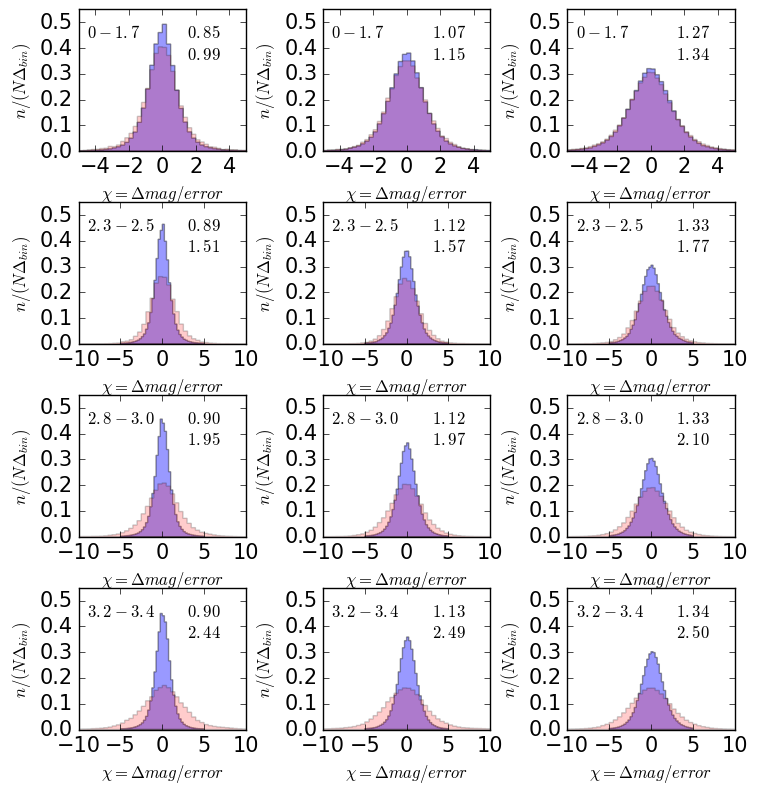
\includegraphics[width=1.1\columnwidth]{Fig_3_histogram_panels_NEW.png}
 \caption{The top panels show how the histogram of  $\chi = \Delta_{m}/ \mathrm{error}$ for small 
timescales ($\log{\Delta_{t}} < 1.7$, $t<50$ days) for  quasars (red) overlaps almost perfectly with blue stars (blue). The  implied small quasar variability is at the level  measured by SDSS.  From left to right, we iterate over the  magnitude bins :  $17-18$,  $18-18.5$, and $18.5-19$ mag. From top to bottom we change the  $\log{\Delta_{t}}$  range. Note how  the  stars, being nonvariable, maintain the same spread of $\chi$, due to their lack of intrinsic variability. The quasars spread more thanks to their intrinsic variability, but at small timescales their spread is same as that of stars, consistent with their lack of short timescale variability. On each plot numbers in the upper-left corner indicate the $\log{\Delta_{t}}$ range, and in the upper-right the robust width of stellar and quasar distributions of $\chi$. }
\end{figure}

\section{Results}
\label{sec:err_analysis}
To study  the intrinsic variability of quasars we use the standard stars that do not exhibit any intrinsic variability as the control sample. We define our sample in a following way: for both stars and quasars, we require SDSS  r-band $17< m_{SDSS,r} < 19$, and the CRTS lightcurve-averaged error  to be   $ <e_{w}> \rangle < 0.3$. To study the structure function and error properties in greater detail we further subdivide this sample into three magnitude bins: 17-18, 18-18.5, and 18.5-19 mag.   To acknowledge the influence of colors on photometric error,  we divide the stars in two color bins: "red" with   $1 < g-i < 3$ and "blue" $-1 < g-i < 1$,  using SDSS $g$ and $i$ filters .  Fig.~\ref{fig:panel_plots}, shows the 18.5-19 mag, which illustrates the problem : nonzero structure function even for the blue stars. Quasars show the SF on the similar level to blue stars.  A quantity $\chi = \Delta_{m}/ \mathrm{error}$, shown on Fig.~\ref{fig:histograms} for four different $\log{\Delta_{t}}$ regimes illustrates the point.  


For each magnitude-$\log{\Delta_{t}}$   bin we calculate a set of properties: the  median CRTS lightcurve error, the robust standard deviation of $\Delta_{m}$,    median CRTS lightcurve day-averaged magnitude, median CRTS lightcurve average error, and the robust standard deviation of  the $\chi$ distribution. For stars, which have no intrinsic variability, the width of $\chi$ distribution should be 1.  Any deviation from that is due to unaccounted errors. For this reason we define the $ f_{c,B}$ - the correction factor from blue stars, as the width of $\chi$ distribution for blue stars in the short timescale bin ($\log{\Delta_{t}} < 1.7$) (see Table~\ref{tab:chi_values} for values of $\chi$ for other bins). Applying thus derived correction factors to the overall sample shows that the structure function for the blue stars is brought to values allowed by the sky photometric variability (0.05 mag level, green dashed line on Fig.~\ref{fig:CRTS_QSO_sample}). Values of $\chi$ for various magnitude-  bins is shown in Tab.~\ref{tab:chi_values} . 



\begin{table}

\caption{Values of $\chi$ for various magnitude- $\log{\Delta_{t}}$ bins for blue stars. }
\label{tab:chi_values}
\begin{tabular}{ l|cccc } 
 \hline
\backslashbox{mag}{$\log{\Delta_{t}}$ }   & 0-1.7 &  2.3-2.5 & 2.8-3.0 & 3.2-3.4 \\ 
 \hline
17-18   & 0.864 &   0.907  & 0.916   & 0.915 \\ 
18-18.5 & 1.091 &   1.143  & 1.150   & 1.160 \\ 
18.5-19 & 1.298 &   1.359  & 1.360   & 1.368 
 \hline
\end{tabular}
\end{table}




\begin{figure}
\label{fig:CRTS_QSO_sample}
 \includegraphics[width=\columnwidth]{{Fig_4_SF_QSO_starsB_r_cut_fc-0.864-1.091-1.298_NEW}.png}
 \caption{Three panels compare the Structure Function (SF)  for quasars and blue stars in three magnitude bins based on their mean SDSS $r$ magnitude. We correct the CRTS errors using listed $fc$ factors. Stars have a flat SF consistent with their lack of  variability, whereas quasars have a nonzero variability. At short time scales, the quasar variability seen in CRTS data is consistent with that from SDSS, shown by horizontal green lines. }
\end{figure}


\section{Conclusions}
\label{sec:conclusions}
CRTS errors were underestimated at the 20-30 \% level.

Implications:  * information from correspondence with M. Graham  
* other recent findings that are based on short timescale CRTS variability  - all would be called into question  



\section*{Acknowledgements}

Funding for the SDSS and SDSS-II has been provided by the Alfred P. Sloan Foundation, the Participating Institutions, the National Science Foundation, the U.S. Department of Energy, the National Aeronautics and Space Administration, the Japanese Monbukagakusho, the Max Planck Society, and the Higher Education Funding Council for England. The SDSS Web Site is http://www.sdss.org/.

The SDSS is managed by the Astrophysical Research Consortium for the Participating Institutions. The Participating Institutions are the American Museum of Natural History, Astrophysical Institute Potsdam, University of Basel, University of Cambridge, Case Western Reserve University, University of Chicago, Drexel University, Fermilab, the Institute for Advanced Study, the Japan Participation Group, Johns Hopkins University, the Joint Institute for Nuclear Astrophysics, the Kavli Institute for Particle Astrophysics and Cosmology, the Korean Scientist Group, the Chinese Academy of Sciences (LAMOST), Los Alamos National Laboratory, the Max-Planck-Institute for Astronomy (MPIA), the Max-Planck-Institute for Astrophysics (MPA), New Mexico State University, Ohio State University, University of Pittsburgh, University of Portsmouth, Princeton University, the United States Naval Observatory, and the University of Washington. 


%%%%%%%%%%%%%%%%%%%%%%%%%%%%%%%%%%%%%%%%%%%%%%%%%%

%%%%%%%%%%%%%%%%%%%% REFERENCES %%%%%%%%%%%%%%%%%%

% The best way to enter references is to use BibTeX:

%\bibliographystyle{mnras}
%\bibliography{example} % if your bibtex file is called example.bib

%%%%%%%%%%%%%%%%%%%%%%%%%%%%%%%%%%%%%%%%%%%%%%%%%%


% Don't change these lines
\bsp	% typesetting comment
\label{lastpage}
\end{document}

% End of mnras_template.tex
